\documentclass[11pt,a4paper,oneside]{book}
\usepackage[a4paper,margin=22mm]{geometry}
\usepackage[T1]{fontenc}
\usepackage{newtxtext,newtxmath}
\usepackage{microtype}
\usepackage{booktabs}
\usepackage{tabularx}
\usepackage{array}
\usepackage{graphicx}
\usepackage{float}
\usepackage{xcolor}
\usepackage{enumitem}
\usepackage[most]{tcolorbox}
\usepackage[hidelinks]{hyperref}
\setlist{itemsep=1pt,topsep=3pt}
\setlist[enumerate]{label=\arabic*.}
\graphicspath{{fig/}}
\newcommand{\Tab}[1]{\begingroup\small\input{tab/tab_#1.tex}\endgroup\par\medskip}
\newcommand{\key}[1]{\texttt{#1}}
\newcommand{\ann}[1]{\textsf{\small #1}}
\newcommand{\Pic}[3][\textwidth]{\begin{figure}[H]\centering\includegraphics[width=#1]{#2}\caption{#3}\end{figure}}
\newtcolorbox{warning}{enhanced,colback=white,colframe=black,boxrule=1.2pt,arc=0pt,left=6pt,right=6pt,top=3pt,bottom=4pt,
  title={\centering\bfseries WARNING},coltitle=black,colbacktitle=white,titlerule=0pt,fonttitle=\normalsize}
\newtcolorbox{caution}{enhanced,colback=white,colframe=black,boxrule=0.6pt,arc=0pt,left=6pt,right=6pt,top=3pt,bottom=4pt,
  title={\centering\bfseries CAUTION},coltitle=black,colbacktitle=white,titlerule=0pt,fonttitle=\normalsize}
\newtcolorbox{note}{enhanced,colback=white,colframe=white,boxrule=0pt,left=6pt,right=6pt,top=2pt,bottom=2pt,
  title={\centering\bfseries Note},coltitle=black,colbacktitle=white,titlerule=0pt,fonttitle=\normalsize}

\begin{document}
\frontmatter
\begin{titlepage}
\centering
\vspace*{40mm}
{\Huge\bfseries X-57 Maxwell\par}
\vspace{6mm}
{\LARGE Flight Manual\par}
\vspace{4mm}
{\large Mod III and Mod IV, for FlightGear with the JSBSim flight model\par}
\vspace{14mm}
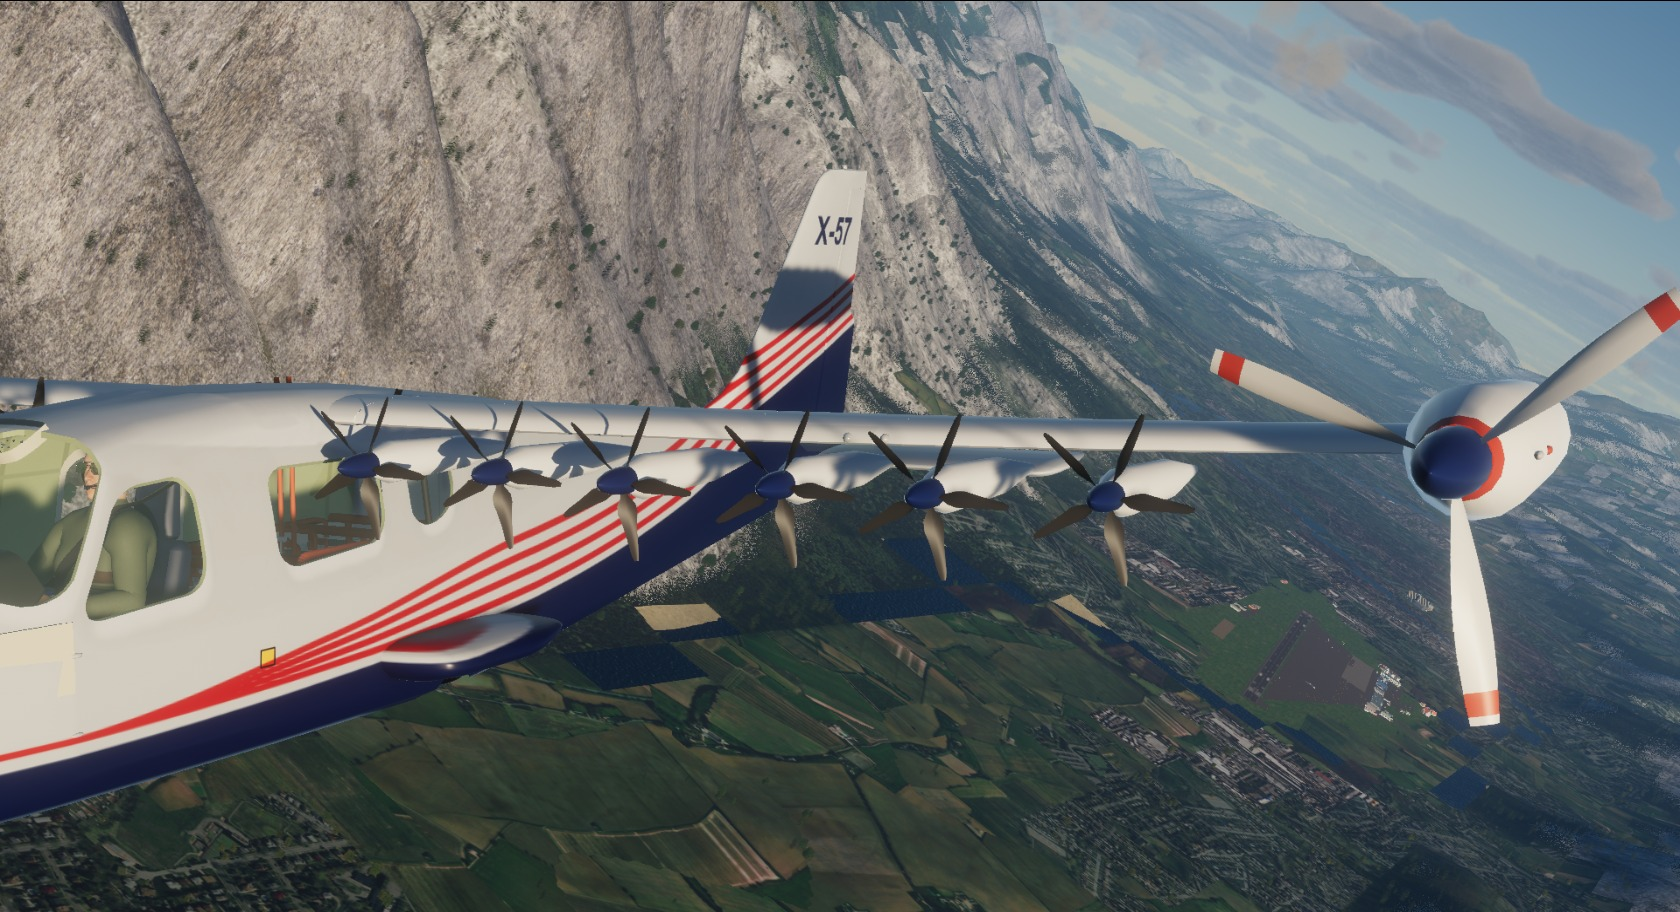
\includegraphics[width=0.8\textwidth]{../X57.jpg}\par
\vspace{14mm}
\begin{minipage}{0.75\textwidth}\small
This manual describes the aircraft as simulated. Mods III and IV never flew, and NASA's own Pilot's Operations Handbook isn't public, so this is not a real
aircraft's manual and its procedures are for the simulator only. It comes from NASA's published Cockpit Interface Control Document and papers and the Tecnam P2006T flight
manual. This work is not connected with or endorsed by NASA or Tecnam.
\end{minipage}
\vfill
{\small Generated from the aircraft's sources (\texttt{manual/} in its repository). November 2026.\par}
\end{titlepage}

\chapter*{How to use this manual}
\addcontentsline{toc}{chapter}{How to use this manual}
The manual runs as a flight manual does: the aircraft, its cockpit and systems, limitations, normal procedures, flight characteristics, emergency procedures and performance. Appendix~\ref{app:icd} sets the cockpit beside NASA's handbook, and lists every place the two differ. Keys are given as \key{g}; words on the panel, as \ann{ESS BATT}.

Performance figures are the model's, with NASA's predictions beside them where there are any. How far to trust each one is in the model's report, \emph{Flight Dynamics of the X-57 Maxwell in JSBSim}.

\paragraph{Warnings, cautions and notes.} Three kinds of notice stand apart from the text, by how much they matter:
\begin{warning}
A procedure or technique that, not followed, may lose the aircraft.
\end{warning}
\begin{caution}
A procedure or technique that, not followed, may damage the aircraft or end the flight's purpose.
\end{caution}
\begin{note}
A procedure, technique or fact worth emphasising.
\end{note}

\tableofcontents
\mainmatter

\chapter{General description}
\section{The aircraft}
The X-57 Maxwell is NASA's battery-electric demonstrator, built on a Tecnam P2006T. Its forms are called Mods:
\begin{description}
\item[Mod II] the P2006T with its piston engines replaced by electric motors. Built and tested on the ground. Not simulated here.
\item[Mod III] a new wing of 42\,\% of the area and aspect ratio 15, with the cruise motors at the tips, where their propellers turn against the tip vortices. The high-lift motors are on it, folded and inactive. The wing was built and tested; the aircraft never flew.
\item[Mod IV] Mod III with twelve folding high-lift propellers along the leading edge, to fly slowly on so small a wing. Never built.
\end{description}
From Mod II on, a flight-test air-data boom of the NACA style projects from the nose's right side, its pitot tip about 1.2\,m ahead; its two vanes, for angle of attack and sideslip, trail into the airflow in flight. Its sizes are estimates from NASA's rendering. Both Mods share this cockpit. On Mod III the high-lift panel stays dark. The cabin is NASA's: one seat, the pilot's. The copilot's seat, yoke and pedals gave way to a research instrumentation pallet, which holds the data logger, and the rear seats to the traction battery modules and their control systems. Their look follows NASA's photographs; their sizes and places are estimates. The pilot's rudder pedals, with toe brakes, swing with the rudder and brakes. Outside the Cockpit View a pilot sits in the left seat, his hands on the yoke and torque levers and his feet on the pedals, following them. He is 1.75\,m tall, on a seat lowered 8\,cm from the P2006T model's place, as the real seat adjusts, and he wears its three-point seatbelt and black work shoes. He wears a headset and green-lensed aviator sunglasses.

\begin{table}[H]\centering\small
\caption{Principal data.}
\begin{tabular}{@{}lll@{}}
\toprule
 & Mod III & Mod IV \\
\midrule
Wing area, span & \multicolumn{2}{l}{66.7\,ft$^2$, 31.6\,ft} \\
Weight flown in FlightGear & 3000\,lb & 3200\,lb (projected) \\
Centre of gravity & \multicolumn{2}{l}{28.6\,\% of the chord: no fuel, so it stays put} \\
Cruise propellers & \multicolumn{2}{l}{two, 3 blades, 1.52\,m, electric variable pitch} \\
Cruise motors & \multicolumn{2}{l}{255\,Nm, 72\,kW at 2700\,rpm, two controllers each} \\
High-lift propellers & twelve, folded, inactive & twelve, 5 blades, 0.58\,m, folding, fixed pitch \\
Traction battery & \multicolumn{2}{l}{two packs, 5120 cells in all, 51.2\,kWh usable} \\
Target cruise & \multicolumn{2}{l}{150\,KTAS at 8000\,ft} \\
\bottomrule
\end{tabular}
\end{table}

\enlargethispage{1\baselineskip}
\section{Controls in FlightGear}
\Tab{keys}
The levers use FlightGear's throttle and propeller pitch controls.

\begin{itemize}
\item \textbf{X-57 menu $>$ Autostart} runs NASA's start-up order in 25 seconds, needed only after shutting down.
\item \textbf{X-57 menu $>$ Autostop} runs the shutdown, on the ground only.
\item \textbf{X-57 menu $>$ Systems and failures} sets NASA's failures and the levers' overdrive and regeneration.
\end{itemize}

\chapter{The cockpit}
\Pic[0.82\textwidth]{pilots-view.jpg}{The pilot's view.}
\Pic{panel.jpg}{The instrument panel.}
\section{Left panel}
\Pic[0.82\textwidth]{panel-left.jpg}{Left panel.}
\Tab{left}
\subsection{High-lift panel (Mod IV)}
\Tab{highlift}
\subsection{Annunciator}\label{sec:ann}
\Tab{annunciator}
Red means act now. Yellow means caution, and return to base if it can't be cleared.

The aural alert repeats every two seconds until acknowledged with \ann{AUDIO ANN. ACK}.

\section{Centre stack}
\Pic[0.82\textwidth]{panel-centre.jpg}{Centre stack.}
\Tab{centre}
\subsection{D175 pages}
\Tab{d175}
The ten lights along the top show CAN bus traffic. From left: left data acquisition, left CMC A and B, left BMS, left torque encoder, right torque encoder, right BMS, right CMC A and B, right data acquisition.
\begin{caution}
NASA treats the D175 as test information only. Trust the energy meters for the battery's state: NASA's state of charge drifts.
\end{caution}

\section{Right panel}
\Pic[0.82\textwidth]{panel-right.jpg}{Right panel.}
\Tab{right}

\section{Overhead and levers}
\Pic[0.82\textwidth]{overhead.jpg}{Overhead panel: the traction battery and contactors.}
\Pic[0.82\textwidth]{pedestal.jpg}{Pedestal: torque and propeller levers.}
\Tab{levers}
FlightGear's throttle stops at idle and full. For regeneration press \key{Delete} (\key{Backspace} on a Mac): the throttles then run from idle at the top to full regeneration at the bottom, more as they come back, and the levers on the pedestal move back past idle with them. Switched on with the throttles at idle, it starts at full: push them up to ease it off. A joystick's reverser button does the same. On a Thrustmaster Warthog throttle, whose axis reads nothing past the idle detent, bind the idle-detent button to Reverser Toggle: each pass over the detent switches regeneration on or off, and the levers set how much. With FlightGear's own Warthog binding that button gives the lever's motor full regeneration while it is held past the detent. Overdrive, and regeneration in the throttle's bottom tenth, are ticked in \textbf{X-57 menu $>$ Systems and failures}.

\section{Lower panels}
\Tab{lower}

\section{Breaker panels}
\Pic[0.82\textwidth]{breakers-left.jpg}{Left breakers, from NASA's photograph, in their cream moulding between the instrument panel and the main door's frame.}
\Pic[0.82\textwidth]{breakers-right.jpg}{Right breakers: names from NASA's power drawing, their order a guess.}
Click a breaker to pull it. Four do something: \ann{LANDING GEAR}, \ann{FLAP MOTOR} and \ann{PROP CONT.\ L} and \ann{R}.

\chapter{Systems}
\section{Propulsion}
Each cruise motor has two controllers, A and B. The torque lever commands torque: 127.5\,Nm a controller at \ann{FULL}, so 255\,Nm a motor. The propeller lever sets rpm through an electric motor in the hub, which turns the blades at only 1 degree a second. In \ann{AUTO} the hub governs above 200\,rpm; in \ann{MAN} the blades move only while \ann{START} or \ann{FEATHER} is held. Past idle, regeneration turns the motors into generators: the propellers windmill, adding drag and charging the battery. NASA never settled its torque (the interface document had none, and Mod IV's values were never set); the model's full regeneration, 38\,Nm a controller, is the power of the CFD's lowest case, 18\,kW a motor.

\section{High lift (Mod IV)}
Twelve motors drive folding propellers, in four groups, A and B on each wing, each with its own contactor. They do nothing unless selected. All six on a wing turn the same way as its cruise propeller, inboard blade rising, and the left wing mirrors the right.
\begin{description}
\item[\ann{FIXED}] 4800\,rpm, for takeoff.
\item[\ann{AIRSPEED}] the speed follows the airspeed schedule, for landing. Below 95\,KEAS the torque rises from 3\,Nm towards 22\,Nm at 58\,KEAS.
\end{description}
Disarmed, the blades fold along the nacelles.

\enlargethispage{1\baselineskip}
\section{Electrical power}
\Tab{power}
The Essential Bus is the last one to lose: with it dead the contactors open and all traction goes. To shed load, turn off \ann{AVIONICS BUS A} and \ann{B} first.


\section{Exterior lights}
\ann{NAV} lights the tip nacelles and tail, \ann{STROBE} flashes the tips and fin top, and \ann{LANDING} and \ann{TAXI} are in the left wing's leading edge, all on DC Converter Bus B. Position lights and strobes start on.

\section{Cockpit lights}\label{sec:cockpitlights}
The X-57 has none. NASA's power drawings keep the P2006T's \ann{INSTR LIGHT} circuit, 5\,A on DC Converter Bus B, collared out; its photograph of the cockpit has blanks where the P2006T has its dimmers, and its own panel where the P2006T's overhead console was. Its flights were to start within an hour of sunrise, and none was flown: the aircraft never reached a full flight configuration.

For flying in the dark, \textbf{X-57 menu $>$ Tecnam cockpit lights (not on the X-57)} fits the lights a P2006T has. Until then nothing of them is in the cockpit. Fitted, they are:
\begin{itemize}
\item \ann{INSTR}, a fifth rocker in the \ann{LIGHTS} row, as on the P2006T: the instrument lights, on DC Converter Bus B through the \ann{INSTR LIGHT} breaker.
\item Three dimmers at the P2006T's place for them, which on the X-57 holds its \ann{EXPERIMENTAL} placard: fitted, they take the placard's place. From the left: the switches' built-in lights, the avionics' key lights, and the cockpit lights, two lamps in the ceiling that light the left and right panels. Drag a knob up or down.
\item The cabin light in the ceiling behind them, on the Essential Bus, its switch on the lamp.
\item The emergency light, five LEDs just aft of the traction power panel, straight from the Essential battery, its switch on the lamp.
\end{itemize}
The places come from the P2006T's flight manual and a model of its overhead console; the levels are estimates. The same switches and dimmers are in the menu's window.

\section{Landing gear and flaps}
The gear is the P2006T's, electro-hydraulic, and takes about 6 seconds. It runs on the Essential Bus. \ann{TRANS} shows it moving, and \ann{GEAR PUMP ON} the pump running. The flaps have one electric motor on the Essential Bus, at 3 degrees a second: 10 for takeoff, 30 for landing.
On the ground the gear stays down whatever the lever says, and comes up as the wheels leave the ground if the lever is up. That guard is a simulator choice: sources disagree on a squat switch.

The pedals move the rudder, 26 degrees each way, and steer the nose wheel with it in proportion, to 20. The linkage has some play: within 2 degrees either side of where the pedals put it, the nose wheel trails. How much play the real aircraft has isn't published; this figure is fitted to NASA's ground simulation. At speed the nose wheel bites hard. In a 15\,kt crosswind from behind, about 3 degrees of nose wheel holds the line; 5 or more above 20\,kt leans the aircraft onto a wingtip propeller.

\chapter{Operating limitations}
\begin{table}[H]\centering\small
\caption{Limits.}
\begin{tabular}{@{}ll@{}}
\toprule
Never exceed speed & 172\,KCAS \\
Propeller speed & 1700 to 2700\,rpm, tachometer red above 3080 \\
Torque & 255\,Nm a motor; 175\,Nm overdrive on one controller, with the other lost \\
High-lift deployment & select \ann{AIRSPEED} above 120\,KEAS, \ann{ARM} between 120 and 95\,KEAS \\
Traction bus & caution at or below 350\,V \\
Traction battery & caution below 310\,V; cell above 65\,\textdegree C is a red alert \\
Essential battery & flashing alert below 12.8\,V \\
Converter output & 13 to 14.6\,V, 0 to 70\,A \\
Ceiling & 14\,000\,ft capable, 10\,000\,ft operational \\
Flap settings & 0, 10, 30 degrees \\
\bottomrule
\end{tabular}
\end{table}
\begin{note}
No gear or flap speed limit is published for the X-57, and the model has none. The P2006T's are 93\,KIAS, which the X-57's own takeoff speeds exceed.
\end{note}

\chapter{Normal procedures}
\section{Start-up}
Everything is on the panel. Each low voltage switch goes up, working from left to right.

\Tab{startup}
\begin{caution}
Before starting a motor the blades must be at \ann{START}, because \ann{AUTO} only works above 200\,rpm. If the green \ann{START} light is out, set \ann{MAN} and hold \ann{START}.
\end{caution}

\section{Takeoff}
\subsection{Speeds}
\Tab{speeds}
\subsection{Mod III}
Flaps 10, full torque, 2700\,rpm. The P2006T's brakes hold the aircraft only to about half torque, so let them off and push the levers up as it rolls. Rotate at 88\,KIAS and climb at 96. Be ready for a long run: about 4300\,ft with the model's automated test pilot. Raise the gear and flaps at a safe height.

\subsection{Mod IV: Distributed Thrust Takeoff (DiTTo)}
DiTTo is a technique for the pilot, not software. Nothing automatic mixes the motors or reacts to the rudder and ailerons. Holding the wingtip motors to about two thirds power keeps a motor failure controllable, and the high-lift motors make up the thrust.
\begin{enumerate}
\item During the run-up at raised torque, set the propeller levers to 1800\,rpm and leave them there.
\item Line up, select \ann{FIXED} and move to \ann{ARM}. All twelve high-lift motors spin up to 4800\,rpm. \ann{RDY} goes out and \ann{RUN} turns green. Their thrust alone, about 750\,lbf, is more than the model's brakes hold, so it starts rolling: arm on the runway, lined up.
\item Push the torque levers to the \ann{FULL} detent, the top of the throttle unless Overdrive is ticked. That's 255\,Nm and about 48\,kW a motor, 67\,\% of rated power.
\item Rotate at 77\,KIAS and climb at 84\,KIAS.
\item At a safe height, accelerate to best rate of climb, then raise gear and flaps and disarm the high-lift motors.
\item Cruise climb at 2250\,rpm and 255\,Nm, about 60\,kW a motor.
\end{enumerate}

\section{Cruise}
At 2250\,rpm, trim and set torque for the speed. 150\,KTAS at 8000\,ft takes about 85\,kW in the model. Watch the energy meters, not the D175's state of charge.

\section{Approach and landing}
\subsection{Mod III}
With no high lift the approach is fast: NASA's reference speed is 94\,KCAS. Gear down, flaps 30.
\subsection{Mod IV}
\begin{enumerate}
\item Select \ann{AIRSPEED} while above 120\,KEAS. In \ann{FIXED} the propellers push harder: at idle the model climbs at 75\,KCAS, and full regeneration gives only 2.6 degrees down.
\item \ann{ARM} between 120 and 95\,KEAS.
\item Gear down, flaps 30, propeller levers forward to 2700\,rpm in case of a go-around, and slow to 75\,KCAS. The high-lift propellers now hold the wing up: the model settles at about 4300\,rpm and 5\,kW a disc.
\item Their thrust works against the descent. With the torque levers at idle the model holds a 3-degree path only at about 78\,KCAS, and slower the path flattens, level near 68. So below about 80\,KCAS on final, hold the path with regeneration: that is what NASA gave the levers' regeneration region, glide path control on a Mod IV approach. Just past idle is enough for 3 degrees at 75\,KCAS: the idle torque gone, the propellers windmill. Full regeneration gives about 5. Fly it like a throttle, more for a steeper path and less for a flatter one. Hold the speed: at 70\,KCAS 3 degrees takes nearly full regeneration, and slower no amount holds it.
\item After touchdown, press the red disarm button on the yoke's left horn. The propellers stop and the blades fold. Until then their thrust outruns the brakes: NASA's pilots found that in the simulator, and the button was added for it.
\item On a go-around: regeneration off (in it, full throttle is only idle), torque levers to \ann{FULL}, and \ann{FIXED}, as NASA planned for a high-performance takeoff. At 75\,KCAS the model then climbs at 12 degrees against 10 in \ann{AIRSPEED}, at a lower angle of attack. Flaps 10 once climbing, then clean up as after takeoff. Disarm above 120\,KEAS and the blades fold.
\end{enumerate}
\begin{warning}
On Mod IV at approach speed the wing is flying on the high-lift propellers. Losing them all takes the stall speed from 58\,KCAS to about 75, Mod III's 73 at this weight: that's the approach speed.
\end{warning}

\section{Shutdown}
Torque levers to idle, disarm left then right, open the contactors, then \ann{MAIN BATT}. Then work the low voltage switches from right to left, with \ann{ESS BATT} last.

\chapter{Flight characteristics}
\section{Modes}
\begin{table}[H]\centering\small
\caption{Mod III's modes in the model, NASA's simulator in brackets.}
\begin{tabular}{@{}lrrr@{}}
\toprule
 & 88\,KCAS & 96\,KCAS & 112\,KCAS \\
\midrule
Phugoid damping ratio & 0.099 (0.104) & 0.104 (0.116) & 0.120 (0.122) \\
Short period damping ratio & 0.361 (0.374) & 0.414 (0.382) & 0.467 (0.439) \\
Dutch roll damping ratio & 0.106 (0.118) & 0.124 (0.136) & 0.157 (0.158) \\
Roll time constant, s & 1.00 (1.03) & 0.81 (0.83) & 0.62 (0.66) \\
\bottomrule
\end{tabular}
\end{table}
The aircraft is lightly damped in yaw, and the roll is slow for its size: the long wing's weight is far out, with a motor at each tip. Near stall the Dutch roll gets much weaker: its damping falls to 0.04 at 80\,KCAS in the model (NASA's simulator 0.11).

\section{Stall}
Mod III stalls fast, and with little to spare: at 3000\,lb the model's trimmed stall speeds are 82.7, 80.6 and 70.8\,KCAS with flaps 0, 10 and 30, NASA's 88, 80 and 73. The high-lift propellers on Mod IV bring it down to 58\,KCAS.

\section{The wing}
The wing bends in its first mode, about 2.4\,Hz up and down together and 3.5 to 3.9\,Hz opposed, with the motors at its tips. It's damped in flight at every speed, lightly: a damping ratio of 0.02 to 0.04.

\section{Sound}
There are no piston engines: what you hear is the electric drive. Each motor whines with its own tones, and the propellers hum at their blade-passing frequencies: the two cruise propellers at the wingtips and, on Mod IV, the twelve high-lift propellers along the leading edge while they're armed. With the motors idling on the ground it's quiet, with the gear pump and flap motor clear; in flight the wind takes over, and at 100\,kt it's about 10\,dB over the two cruise propellers together. In flight the flap motor can't be heard in the cockpit, and the gear pump is faint. Outside, the gear out at 90\,kt is about as loud as a cruise propeller. See appendix~\ref{app:sound}.

\chapter{Emergency procedures}
NASA's emergency procedures aren't public. Those here come from its papers where it says so, and otherwise are this manual's own, from what each failure does.
\section{Motors and propellers}
\subsection{A cruise motor lost}
The motor at the wingtip has a long arm. Left alone, in the model the aircraft rolls past 79 degrees in 3 seconds at 95\,KCAS, with a peak roll rate of 49 degrees a second: about three times as hard as a Mod II.
\begin{warning}
Below minimum control speed (Mod III 85\,KCAS, the model 84.1) full rudder won't hold the aircraft at full power on the good side. Pull the torque lever back to cut the asymmetry.
\end{warning}
\begin{enumerate}
\item Aileron and rudder against the roll, at once.
\item Good motor's torque lever back if needed to hold control.
\item Lower the nose, and hold at least 96\,KIAS.
\item Failed side's propeller lever to \ann{FEATHER}, to stop the dead propeller windmilling. The blades turn only 1 degree a second, so this takes over a minute, and until it's done the drag costs about 110\,ft/min more.
\end{enumerate}
With a motor out and feathered, gear down and takeoff flaps, Mod III at 97\,KCAS sinks about 420\,ft/min, so it won't climb away like that.

\subsection{Runaway propeller}
NASA's emergency stop for a runaway propeller is to pull \ann{PROP CONT.\ L} or \ann{R}, which freezes that hub.

\subsection{High-lift motors lost (Mod IV)}
If high-lift motors fail on one side, press the yoke's disarm button (\key{Y}) to remove the asymmetry, as NASA's pilots did in the simulator. \ann{RESET REQ'D} lights: move \ann{ARM} to \ann{DISARM/RESET}.
\begin{warning}
A contactor failure takes three discs on one wing at once, costing about 0.3 to 0.4 of the lift coefficient at 58\,KCAS and rolling the aircraft. Add speed.
\end{warning}

\section{Electrical and battery}
\subsection{Emergency shutdown}
Torque levers to idle, propeller levers to feather, \ann{MAIN BATT A} and \ann{B} off. Then \ann{CROSS BUS A} and \ann{B}, \ann{DC CONV A} and \ann{B}, and \ann{ESS BATT} as soon as practical.

\subsection{Annunciator alerts}
\begin{table}[H]\centering\small
\begin{tabularx}{\textwidth}{@{}lX@{}}
\toprule
Alert & Action \\
\midrule
\ann{MAIN BATT A}, \ann{B} (red) & Cell above 65\,\textdegree C: reduce power, land now. If it goes on rising, emergency shutdown \\
\ann{ESS BATT} (red) & Battery failed or below 12.8\,V: check the cross buses and converters. Shed \ann{AVIONICS BUS A}, \ann{B}. With the Essential Bus dead all traction goes \\
\ann{TRAC BUS A}, \ann{B} (yellow) & At or below 350\,V: reduce power, return to base \\
\ann{DC CONV A}, \ann{B} (yellow) & Converter failed, or traction battery below 310\,V: return to base \\
\ann{LEFT}, \ann{RIGHT CMC A}, \ann{B} (yellow) & Controller failed, or armed with no traction voltage: that motor has half its torque or less \\
\ann{MAIN DOOR OPEN}, \ann{REAR DOOR OPEN} (red) & Land and close it \\
\bottomrule
\end{tabularx}
\end{table}

\chapter{Performance data}
All at standard conditions. The model's figures first, NASA's in brackets. Mod III at 3000\,lb for the stalls and cruise, 3075\,lb for the climbs, as NASA's simulator.

\begin{table}[H]\centering\small
\caption{Rates of climb, gear down, takeoff flaps, 2500\,ft, ft/min.}
\begin{tabular}{@{}lr@{}}
\toprule
Mod III, 97\,KCAS, full power & 597 (430) \\
Mod III, 97\,KCAS, 2400\,rpm & 426 (270) \\
Mod III, a motor out and feathered & $-418$ ($-450$) \\
Mod III, a traction bus out & $-315$ ($-300$) \\
Mod IV, DiTTo, 97\,KIAS, all working & 787 (720) \\
Mod IV, DiTTo, 97\,KIAS, a motor out & 86 (360) \\
Mod IV, DiTTo, 97\,KIAS, a contactor out & 599 (480) \\
Mod IV, DiTTo, 97\,KIAS, a traction bus out & $-174$ ($-100$) \\
Mod IV, DiTTo, 84\,KIAS, all working & 1151 (1000) \\
Mod IV, DiTTo, 84\,KIAS, a motor out & 455 (530) \\
Mod IV, DiTTo, 84\,KIAS, a contactor out & 893 (740) \\
Mod IV, DiTTo, 84\,KIAS, a traction bus out & 87 (100) \\
\bottomrule
\end{tabular}
\end{table}

\begin{table}[H]\centering\small
\caption{Other figures.}
\begin{tabular}{@{}lr@{}}
\toprule
Lift-to-drag ratio at 150\,KTAS, 8000\,ft & 14.2 (13.5) \\
Best lift-to-drag ratio, at 110\,KCAS & 15.6 (15.9) \\
Power for 150\,KTAS, 8000\,ft & 82\,kW \\
NASA's slow-flight mission, energy drawn & 41.9\,kWh (41.9) of 51.2 usable, in 28 minutes \\
Lowest voltage on that mission & 378\,V (370) \\
Hottest pack on that mission & 59.3\,\textdegree C (57.9) \\
Automated test pilot's takeoff, Mod III & lift-off after 38.9\,s, 3840\,ft, 90\,KCAS \\
Automated test pilot's takeoff, Mod IV & lift-off after 12.3\,s, 1190\,ft, 83\,KCAS \\
\bottomrule
\end{tabular}
\end{table}
\begin{note}
The biggest gaps with NASA are the DiTTo climbs with a motor out. NASA's climb figures imply a smaller loss than its own motor tables give, and the model follows the tables. The aircraft never flew, so nobody can say which figure is right.
\end{note}

\appendix
\chapter{The cockpit and NASA's handbook}\label{app:icd}
NASA's cockpit handbook is public: \emph{X-57 Cockpit Interface Control Document}, ICD-CEPT-006 rev.~E, at \url{https://ntrs.nasa.gov/citations/20230016539}. Read it beside the simulator: this cockpit follows it control by control: names, places, lights and sequences. A check confirms that each of the 119 clickable controls reaches its object and its logic: 113, and six for the Tecnam's cockpit lights. Where the handbook and this model differ, it's listed here.

\section{Differences}
\begin{itemize}
\item The aural alerts are one tone in place of NASA's six spoken messages, whose wording isn't published.
\item The power system runs at fixed voltages, with no sag. Bus loads and the essential battery's 20\,Ah are estimates.
\item Motor and controller temperatures aren't modelled, so those D175 pages show dashes. Battery temperature is.
\item NASA's controllers limit how fast torque changes, but the limit isn't published. The simulator takes one second for the full range, an estimate.
\item Controller lights cover failures and arming without traction voltage, not internal faults.
\item The cabin fan and most breakers have no effect. \ann{PITOT HEAT} isn't modelled.
\item The audio panel isn't modelled. The navigator shows COM~2 and NAV~1 frequencies only, and the transponder its code.
\item The exterior lights work, though NASA's power drawings collar out landing, taxi and nav, the drawing with the Mod IV additions included. All four are on DC Converter Bus B in those drawings. The drawings don't say where the lights sit. Landing and taxi are in the left wing's leading edge, where NASA's photographs show them on Mod II's stock wing. No source shows them on the Mod III wing, so they keep the same distance from the centreline, which puts them behind the fourth high-lift propeller on Mod IV.
\item The cockpit has no lights, as on NASA's aircraft. The P2006T's set can be fitted from the menu: section~\ref{sec:cockpitlights}.
\item FlightGear's controls can't lock a switch, so the lever locks aren't modelled.
\item The gear's ground guard is a simulator choice (see Landing gear and flaps).
\item The right breaker panel's order is a guess, from NASA's power drawing.
\item Mod III shares this cockpit, so its high-lift controls are there but do nothing.
\item The attitude, heading, turn, airspeed, altimeter and climb instruments are the stock P2006T's.
\end{itemize}

\chapter{Sound levels}\label{app:sound}
Every sound plays on one scale, so the balance between them is the physics', as far as it's known. The levels below are A-weighted, in the cockpit and 30\,m outside.
\begin{table}[H]\centering\small
\caption{The airframe's sounds.}
\begin{tabularx}{\textwidth}{@{}lrrX@{}}
\toprule
Sound & Cockpit & 30\,m & Where the level comes from \\
\midrule
Gear pump and jacks & 75 & 30 & estimate, from hydraulic power units' published 58 to 75 at 1\,m \\
Gear locking down, up & 85, 82.5 & 55, 52.5 & estimate, as the ASK~21's airbrake lock \\
Flap motor & 65 & 30 & estimate, from electric actuators' published 55 to 70 \\
Three tyres rolling at 60\,kt & 89.5 & 67 & computed: outside within 0.5\,dB of a towed light aircraft's; inside from a recorded P2006T landing, set against the wind, perhaps up to 3\,dB loud. Each wheel by its own speed \\
A main wheel's touchdown squeal at 60\,kt of slip & 83 & 68 & computed: the energy the tyre loses spinning up, by physics; the share heard and its spectrum from a recorded P2006T landing. Sound exposure, as it's a short event: a firm touchdown is shorter, as loud, and the squeal follows the wheel's load as the recorded one does. The nose wheel's is 79 and 67. A wheel still turning, after a hop, is quiet \\
A main strut's thump, 0.25 to 1\,ft/s & 69--81 & & estimate: barely heard in the same landing. Plays at its estimate; a firmer one is held under full scale, 3\,dB under it at 2\,ft/s and 7 at 4. Sound exposure \\
Toggle or rocker switch & 78 & & estimate, the loudest 125\,ms \\
Push button, breaker, knob & 72 & & estimate, a lighter mechanism \\
Aural alert & 105 & & 15\,dB over the cockpit's noise at 100\,kt, after ISO~7731 \\
\bottomrule
\end{tabularx}
\end{table}
The propellers, motors, the wind, the gear in the airflow, the tyres rolling and the touchdowns are computed by PyWopWop. The gear in the airflow is Fink's method, the same as for the ASK~21's fixed wheels: at 90\,kt, 73 in the cockpit and 67 at 30\,m. Nobody has heard these aircraft, so none of it has been checked against a recording of them; the tyres and touchdowns take their cockpit levels from a recorded P2006T landing. The wind (91 at 110\,kt) and the motors are the least certain.

\chapter{Sources}
\begin{itemize}
\item X-57 Cockpit Interface Control Document, ICD-CEPT-006 rev.~E: \url{https://ntrs.nasa.gov/citations/20230016539}
\item Power System Human Machine Interfaces for the X-57 Mod II Aircraft: \url{https://ntrs.nasa.gov/citations/20240006533}
\item X-57 Traction Power and Command Systems Development, NTRS 20240009560
\item X-57 Cockpit Display System Development and Features, NTRS 20230005312
\item Flight-Test Approach for X-57 Mod II Configuration, NTRS 20240007413
\item X-57 Flight Systems Integration Path, NTRS 20240005892
\item Distributed Thrust Takeoff for the NASA X-57 Mod IV Flight Demonstrator, NTRS 20240010539
\item Development of the X-57 Mod III/IV Piloted Simulator and Discussion of the Resultant Flying Qualities Predictions, NTRS 20240006496
\item Mitigation of High Lateral Asymmetry Rates Due to Loss of a Cruise Motor on the X-57 Mod III Aircraft, NTRS 20240006682
\item X-57 Flight Controls Lessons Learned: \url{https://ntrs.nasa.gov/citations/20240014847}
\item Tecnam P2006T Aircraft Flight Manual, Doc.\ No.\ 2006/044
\end{itemize}
\end{document}
